\section{Results}
\label{sec:results}

\begin{table*}[tb]
  \caption{Objects} \label{tab:objects} \centering
  \begin{tabular}{|c|l|c|c|c|l|}
    \hline
    &Description& Weight(Kg)&No.Trials&No.Failures&Contains \\
    %&Object& W(Kg)&Trials&Fail&Contains \\
    \hline
    1&White Bottle        & 0.265 & 22& 0 & Vitamins\\
    2&White Porcelain cup & 0.255 & 24& 1 & Nothing\\
    3&Startbucks cup      & 0.220 & 24& 4 & Bolts \\
    4&Nesquick box        & 0.240 & 24& 2 & Nesquick powder\\

    \hline
  \end{tabular}
\end{table*}

\begin{figure*}[tbp]
\centerline{
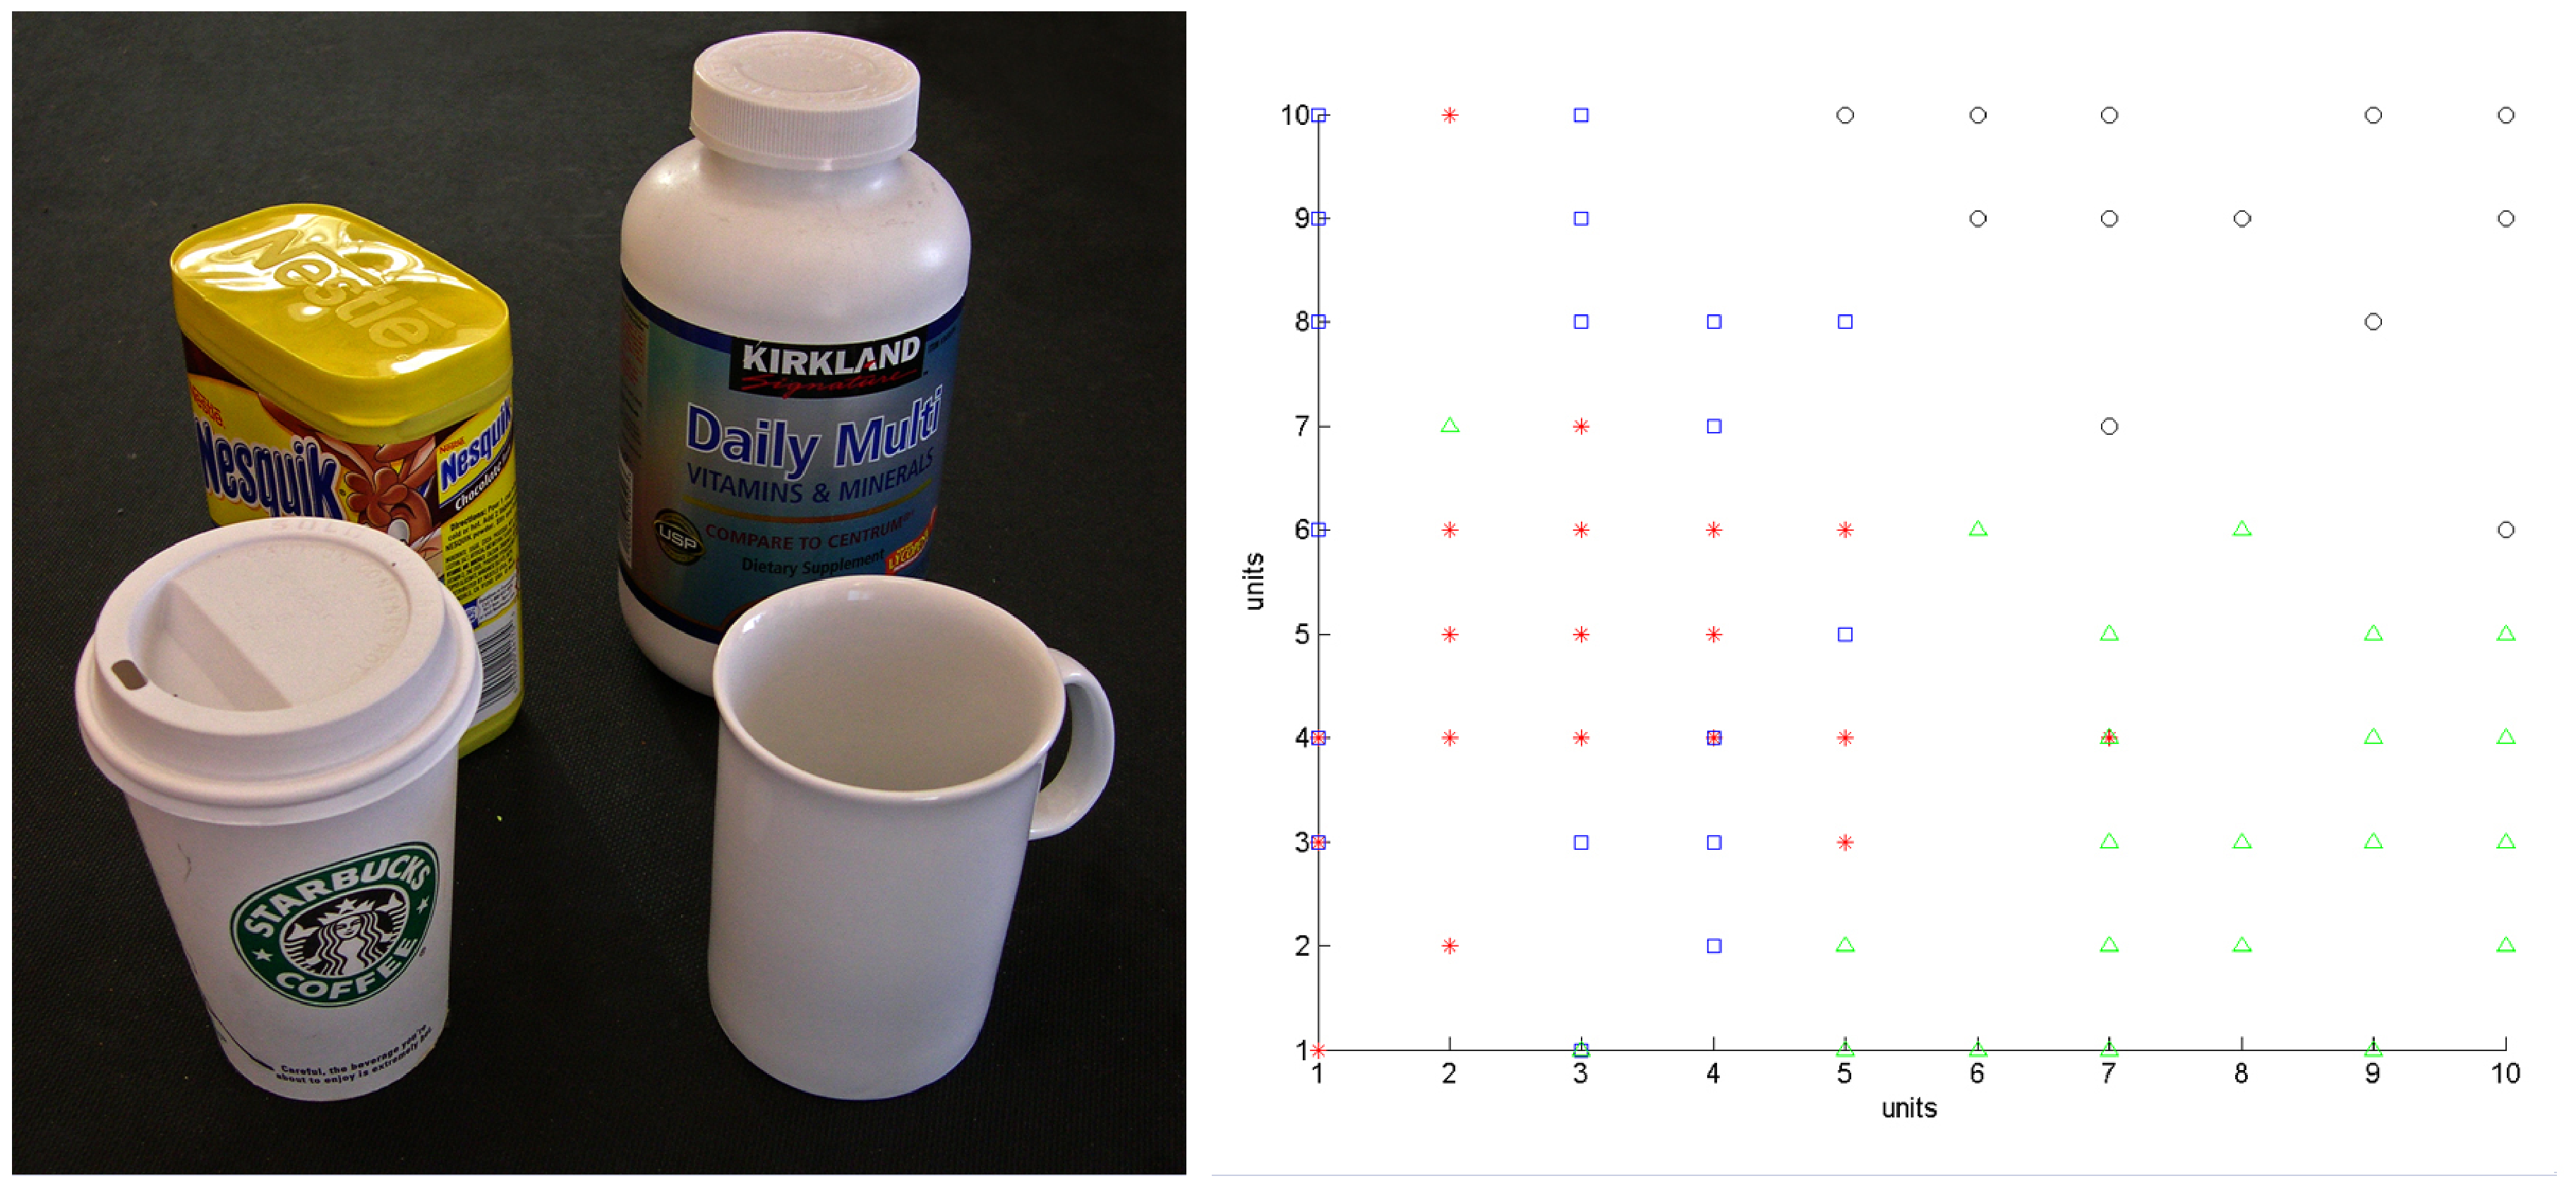
\includegraphics[width=6.0in]{./figures/objects-clusters.eps}
}\caption{Left: the set of objects used in the experiments: a plastic bottle,
a porcelain cup, a plastic cup and a rectangular plastic box. Some objects were
partially filled to increase the weight (all objects weighed about 220-250g).
Right: result of the clustering. Black circles, green
triangles, red stars and blue squares represent respectively the bottle,
the rectangular box and the porcelain and the plastic cups. The two cups are not
clearly separated because have similar shape in the area where they were grasped.}
\label{fig:Objects}
\end{figure*}

%% \begin{figure}[tbp]
%% \centerline{
%% 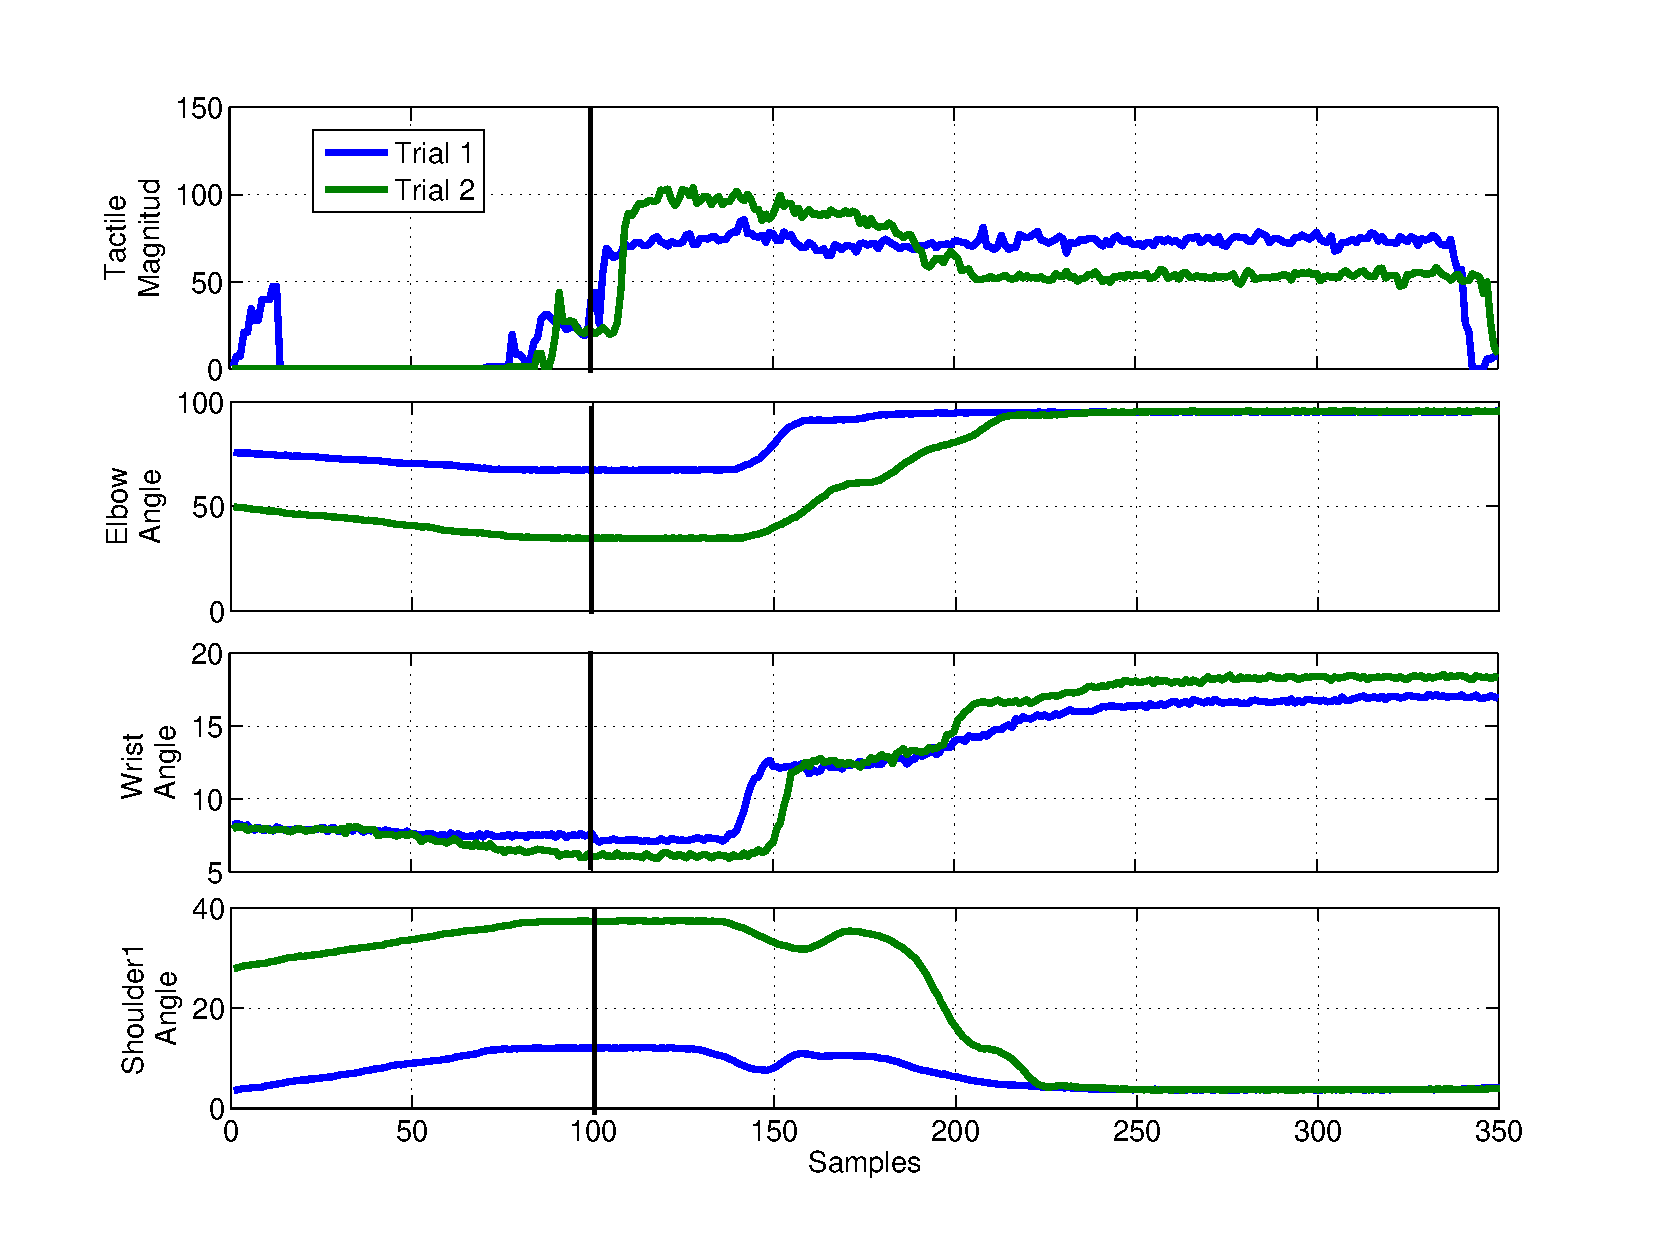
\includegraphics[width=3.5in]{./figures/GraspingData1.eps}
%% }\caption{The figure presents the trajectories followed by two
%% different grasping sequences of a same object. We can observe that
%% the tactile sensor response capture the variation in the different
%% trajectories. The magnitude of the tactile vector is the vectorial
%% summation of the forces present in each tactile sensor considering
%% the current geometry of the hand.} \label{fig:AnglesPlot}
%% \end{figure}

%% \begin{figure}[tbp]
%% \centerline{
%% 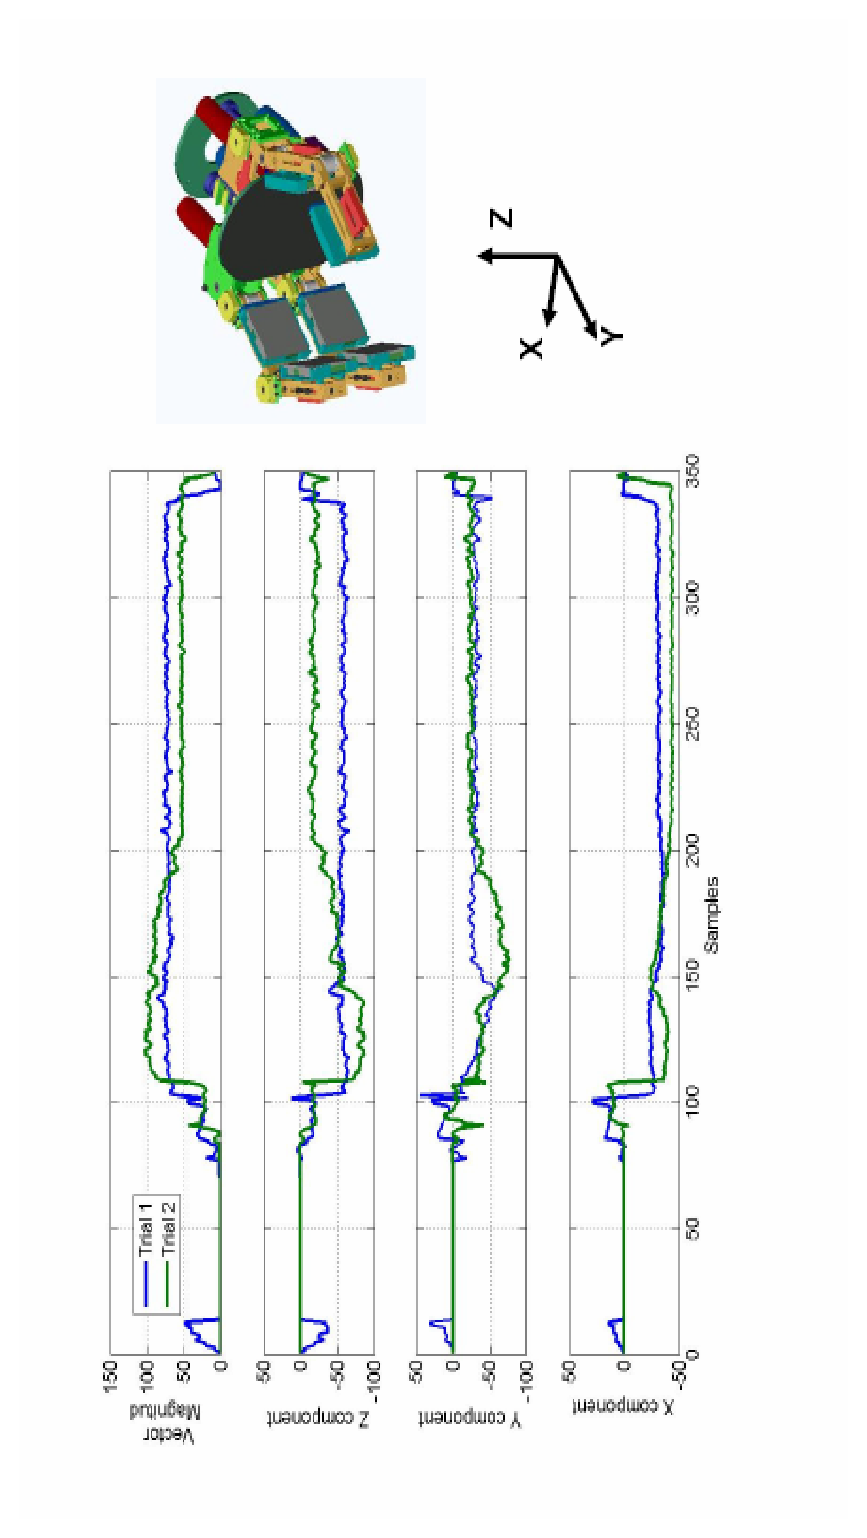
\includegraphics[height=3.2in, angle=270]{./figures/TactileComp.eps}
%% }\caption{The magnitude of the tactile vector is the vectorial
%% summation of the forces present in each tactile sensor considering
%% the current geometry of the hand.} \label{fig:TactileComp}
%% \end{figure}

The grasping behavior section~\ref{sec:controlling} was evaluated 
by presenting different objects to the robot and by counting the 
number of successful grasps.
We chose objects of different size and shape: a plastic bottle, 
a plastic rectangular box, a porcelain cup and a plastic cup 
(see figure~\ref{fig:Objects}. Some of the objects were partially
filled, so that the weight was roughly uniform among all objects 
(about 220-250 grams). The robot had no prior knowledge about the objects.

Each object was presented to the robot more than 20 times and randomly placed
on the table. Overall the number of grasping trials was 94, of which only
6 were not successful. In some of these
trials, the robot managed to grasp the object, but was not able to hold it
because the grip did not produce enough friction. In a few cases the
tactile sensors failed to detect the object and the exploration was aborted
before the object was actually grasped.

As a further validation we clustered the haptic information originated from
the grasping. We collected the hand feedback at the moment the robot lifted the
object; the idea is that given the intrinsic compliance of the hand, its
configuration and the force exerted by each joint depend on the shape of the
object being grasped.
The hand feedback was clustered by means of a Self Organizing Map (SOM). The results
show that the bottle, the rectangular box and the cups form three clusters.
Unfortunately the clusters formed by the two cups are not clearly distinguishable.
This is probably due to the fact that the hand grasped the objects from the
top, and that in that part the two objects are quite alike (both are circular with
similar diameter). In these cases the limited number of fingers (three)
made it hard to distinguish between the cylindrical and conic shape of the cups.
Together the results prove that the grasping behavior of
the robot is reliable. The high number of successful trials shows that the haptic
feedback manages to drive the robot during the exploration until it
finds the object and grasps it. This is further demonstrated by the clustering,
which show that the behavior allows extracting meaningful information about the
physical properties of the objects (i.e. their shape).

%Using the behavior described in section~\ref{}, the robot was able
%to grasp a number of different objects. The robot had no prior
%knowledge of the objects. We evaluate the performance by
%presenting to the robot many times four objects and counting the
%number of times that they were grabbed. Out of 94 trials only 8
%failed. The objects were : a white vitamins bottle, a white
%porcelain cup, a startbucks cup and a nesquick box. The physical
%properties of the objects and the results are shown in table
%\ref{tab:objects}.

%We evaluated our work by performing an object recognition
%experiment. We exposed the robot one evening to a set of seven
%objects, and then in the morning tested its ability to recognize
%another set, which had an overlap of four objects with the
%training set. Three of these objects were chosen (Figure 8) to
%represent three different materials, plastic, glass and steel
%(metal). The idea is that the sound produced by each object
%depends on its size, shape and the material with which it is made;
%accordingly we expected the tapping to produce three different
%distinct sounds. A fourth object (a plastic toy) was relatively
%silent. For each run, we placed randomly selected objects on the
%table in front of the robot, and it was responsible for finding
%and tapping them. Overall the robot tapped 53 times; of these
%episodes 39 were successful, meaning that the sound produced by
%the tapping was significantly loud; in the other 14 cases the
%tapping did not provoke useful events either because the initial
%impact caused the object to fall, or the object remained too close
%to the hand. The high number of successful trials shows that given
%the mechanical design of the hand, haptic feedback was sufficient
%to control the interaction between the robot and the environment.
%We evaluated the performance of our spectrum comparison method by
%ranking the strength of matches between episodes on the second day
%and episodes on the first day. Figure 7 shows what detection
%accuracy is possible as the acceptable false positive rate is
%varied. This predicts that we can on average correctly match an
%episode with 50\% of previous episodes involving the same object
%if we are willing to accept 5\% false matches.
